\documentclass[twocolumn,a4paper]{IEEEtranfr}
%\documentclass
% verbatim : pour afficher le contenu d'un fichier 
%
\usepackage{verbatim}
% gère les graphiques .jpg, .png ,\dots.
\usepackage[dvips]{graphicx}
%
% Pour la gestion de la couleur 
%
\usepackage{color}

%
% Formule chimique
%
\usepackage{chemfig}
%
% + de maths avec AMS
%

\usepackage{amsmath}
\usepackage{amssymb}
%
% Pour afficher des algorithmes
%
\usepackage{algorithm}
\usepackage{algorithmic}
\usepackage{listings}
%
% pour l'hypertexte
%
\usepackage{url}
\usepackage{hyperref}
% français
\usepackage[french]{babel}
% accents
%
% ucs 
% utf8x 
% 
\usepackage{ucs}
\usepackage[utf8x]{inputenc}
%\usepackage[T1]{fontenc}
\usepackage{subfigure}
\usepackage{framed}

\makeatother
% Placer vos figures et images dans les répertoires suivants
% Ne jamais mettre les noms de 
%
% Attention le / final est important 
\graphicspath{{./images/}{./figures/}{../presentation/images/}}

% alias
%
% A consommer sans modération
%
%

\newcommand{\blst}{\begin{lstlisting}}
\newcommand{\elst}{\end{lstlisting}}
\newcommand{\beqan}{\begin{eqnarray*}}
\newcommand{\eeqan}{\end{eqnarray*}}
\newcommand{\beqa}{\begin{eqnarray}}
\newcommand{\eeqa}{\end{eqnarray}}
\newcommand{\bear}{\begin{eqnarray}}
\newcommand{\ear}{\end{eqnarray}}
\newcommand{\bears}{\begin{eqnarray*}}
\newcommand{\ears}{\end{eqnarray*}}
\newcommand{\beq}{\begin{equation}}
\newcommand{\eeq}{\end{equation}}
\newcommand{\rref}[1]{(\ref{#1})}
\newcommand{\eref}[1]{\rref{#1}}
\newcommand{\gd}{\stackrel{.}{\geq}}
\newcommand{\ld}{\stackrel{.}{\leq}}
%%\newcommand{\eqref}[1]{(\ref{#1})}
\renewcommand{\r}{\right}
\renewcommand{\l}{\left}
\newcommand{\lbr}{\left \{ }
\newcommand{\rbr}{\right \} }
\newcommand{\Lbr}{\left [}
\newcommand{\Rbr}{\right ]}
\newcommand{\lp}{\left (}
\newcommand{\rp}{\right )}
%\newcommand{\mylabel}[1]{\label{#1}  \mbox{~~ \tiny \bf [ #1 ] } }
\newcommand{\mylabel}{\label}

%% Notations d'ensembles
\newcommand{\X}{{\cal X}}
\newcommand{\Y}{{\cal Y}}
%\newcommand{\C}{{\cal C}}
\newcommand{\D}{{\cal D}}
\renewcommand{\S}{{\cal S}}
\newcommand{\T}{{\cal T}}
\newcommand{\R}{{\cal R}}
\renewcommand{\H}{{\cal H}}
\newcommand{\V}{{\cal V}}
\renewcommand{\P}{{\cal P}}

%% variables
\newcommand{\eps}{\epsilon}
\newcommand{\real}{{\mathcal {R}}}
\newcommand{\complex}{{\mathcal {C}}}

%% scalaires
\newcommand{\err}{\mathcal{E}}
\newcommand{\dmin}{D_{\min}}
\newcommand{\dl}{D_\ell}
\newcommand{\tw}{\tilde{w}}
\newcommand{\tx}{\tilde{x}}
\newcommand{\ty}{\tilde{y}}
\newcommand{\ha}{h^a}
\newcommand{\dftd}{\tilde{d}}
\newcommand{\dftw}{\tilde{w}}
\newcommand{\dfty}{\tilde{y}}
\newcommand{\dfth}{\tilde{h}}
\newcommand{\Lagrange}{{\mathcal L}}
\newcommand{\Ntones}{N_c}
\newcommand{\hk}{h^{(k)}}
\newcommand{\rh}{{\tt h}}
%%\renewcommand{\ell}{l}

%% vecteurs
\newcommand{\vR}{{\bf R}}
\newcommand{\vmu}{\mbox{\boldmath$\mu$}}
\newcommand{\vbreve}[1]{\v{#1}}
%\renewcommand{\v}[1]{{\bf #1}}
\newcommand{\xmmse}{\hat{\vx}_{{\rm mmse}}}
\newcommand{\va}{{\bf a}}
\newcommand{\vone}{{\bf 1}}
\newcommand{\vb}{{\bf b}}
\newcommand{\vm}{{\bf m}}
\newcommand{\vw}{{\bf w}}
\newcommand{\vwul}{{{\bf w}_{\rm ul}}}
\newcommand{\wul}{{{w}_{\rm ul}}}
\newcommand{\vwdl}{{{\bf w}_{\rm dl}}}
\newcommand{\wdl}{{{w}_{\rm dl}}}
\newcommand{\vs}{{\bf s}}
\newcommand{\vy}{{\bf y}}
\newcommand{\vyul}{{{\bf y}_{\rm ul}}}
\newcommand{\yul}{{{y}_{\rm ul}}}
\newcommand{\pul}{{{P}_{\rm ul}}}
\newcommand{\vydl}{{{\bf y}_{\rm dl}}}
\newcommand{\ydl}{{{y}_{\rm dl}}}
\newcommand{\pdl}{{{P}_{\rm dl}}}
\newcommand{\vz}{{\bf z}}
\newcommand{\vr}{{\bf r}}
\newcommand{\vc}{{\bf c}}
\newcommand{\vh}{{\bf h}}
\newcommand{\vg}{{\bf g}}
\newcommand{\vx}{{\bf x}}
\newcommand{\vxul}{{\bf x}_{\rm ul}}
\newcommand{\xul}{{x}_{\rm ul}}
\newcommand{\vxdl}{{\bf x}_{\rm dl}}
\newcommand{\xdl}{{x}_{\rm dl}}
\newcommand{\vd}{{\bf d}}
\newcommand{\ve}{{\bf e}}
\newcommand{\vv}{{\bf v}}
\newcommand{\vt}{{\bf t}}
\newcommand{\vu}{{\bf u}}
\newcommand{\vP}{{\bf P}}
\newcommand{\vq}{{\bf q}}
\newcommand{\vp}{{\bf p}}
%\newcommand{\vg}{{\bf g}}
\newcommand{\vxN}{{\bf x}^{\bf N}}
\newcommand{\vyN}{{\bf y}^{\bf N}}
\newcommand{\tvw}{{\bf \tilde{w}}}
\newcommand{\tvx}{{\bf \tilde{x}}}
\newcommand{\tvy}{{\bf \tilde{y}}}
\newcommand{\tty}{y'}
\newcommand{\vxa}{{\bf x}^{\bf a}}
\newcommand{\vya}{{\bf y}^{\bf a}}
\newcommand{\vwa}{{\bf w}^{\bf a}}
\newcommand{\var}{{\bf e}_{\bf r}}
\newcommand{\vat}{{\bf e}_{\bf t}}
\newcommand{\vD}{{\bf D}}
\newcommand{\vY}{{\bf Y}}
\newcommand{\vW}{{\bf W}}
\newcommand{\vdftd}{{\bf \tilde{d}}}
\newcommand{\vdftw}{{\bf \tilde{w}}}
\newcommand{\vdfty}{{\bf \tilde{y}}}
\newcommand{\vdfth}{{\bf\tilde{h}}}
\newcommand{\dftmH}{{\bf \tilde{H}}}
\newcommand{\vdftx}{{\bf \tilde{x}}}
\newcommand{\vdfta}{{\bf \tilde{a}}}
\newcommand{\vxA}{{\bf x}^{\bf A}}
\newcommand{\vxB}{{\bf x}^{\bf B}}
\newcommand{\vxAl}{{\bf x}^{\bf A}_{\bf \ell}}
\newcommand{\vxBl}{{\bf x}^{\bf B}_{\bf \ell}}
\newcommand{\rl}{r^{(\ell)}}
\newcommand{\wl}{w^{(\ell)}}
%% matrices
\newcommand{\mQ}{{\bf Q}}
\newcommand{\mU}{{\bf U}}
\newcommand{\mV}{{\bf V}}
\newcommand{\mPsi}{{\bf \Psi}}
\newcommand{\mUt}{{\bf U}_t}
\newcommand{\mUr}{{\bf U}_r}
\newcommand{\mX}{{\bf X}}
\newcommand{\mLambda}{\mathbf{\Lambda}}
\newcommand{\mF}{{\bf F}}
\newcommand{\mK}{{\bf K}}
\newcommand{\mG}{{\bf G}}
\newcommand{\mA}{{\bf A}}
\newcommand{\mB}{{\bf B}}
\newcommand{\mC}{{\bf C}}
\newcommand{\mD}{{\bf D}}
\newcommand{\mR}{{\bf R}}
\newcommand{\mH}{{\bf H}}
\newcommand{\mHa}{{\bf H^a}}
\newcommand{\mI}{{\bf I}}
\newcommand{\mk}{{\bf K}}
\newcommand{\mv}{{\bf V}}
\newcommand{\mO}{{\bf O}} %% orthogonal 
\newcommand{\mJ}{{\bf J}} %% pseudo covariance
\newcommand{\rH}{{\tt H}}
%%\newcommand{\dftmH}{\tilde{\mH}}
\newcommand{\sm}[1]{\sum_{#1=-\infty}^{+\infty}}
\newcommand{\smr}[3]{\sum_{#1=#2}^{#3}}
\newcommand{\smu}[1]{\sum_{#1=1}^{+\infty}}
\newcommand{\smz}[1]{\sum_{#1=1}^{+\infty}}
\newcommand{\ejm}[1]{e^{-j\omega #1}}
\newcommand{\ejp}[1]{e^{j\omega #1}}
\newcommand{\usdp}{\frac{1}{2\pi}}
\newcommand{\edjm}[1]{e^{-j 2\pi f #1}}
\newcommand{\edjp}[1]{e^{j 2\pi f #1}}
%% math notation
\newcommand{\sinc}{{\rm sinc}}
\newcommand{\CN}{\mathcal{CN}}
\newcommand{\N}{\mathcal{N}}
\newcommand{\indistrib}{\stackrel{\mathcal{D}}{\rightarrow}} 
\newcommand{\inprob}{\stackrel{\mathcal{P}}{\rightarrow}}   
\newcommand{\mc}[1]{\mathcal{#1}}

%
%
%  Début du document 
%
%
\begin{document}

\title{Etude et mise en place d'Edge Node sur la base d'OpenEdgeComputing}
\author{HOANG Tuan Dung, KAF Merwan, LE CORRE Pierre} 

% place le titre 
\maketitle

\begin{abstract}
Avec l’arrivée massive des objets connectés, la bande passante du réseau internet risque d'être saturé par la trop grande demande de ressources faites aux serveurs situés dans le Cloud. Afin de palier à ce problème, Orange Labs nous a demandé d'étudier une des solutions existantes : Open Edge Computing. Cette solution consiste à se servir de la puissance de calculs de machines situés en périphérie du réseau (mini datacenter, livebox, ...) afin de permettre aux objets connectés d'accéder à de la puissance de calculs sans remonter jusqu'au serveurs situés dans le cloud. Il nous a ensuite été demandé de nous pencher sur l'implémentation d'une telle solution et d'en estimer la viabilité. 

\end{abstract} 

\begin{keywords}
Cloudlet, Edge Node, Open Edge Computing, Open Stack, Cloud, Virtualisation, Zeroconf
\end{keywords}

%\markboth{This is for left pages}{and this is for right pages}


\section{Introduction}

Le projet que nous a confié la société Orange s’inscrit dans l’anticipation de la multiplication future des objets connectés à internet. Ces derniers utilisent la puissance de calculs de serveurs distants très haut dans le réseau - que l’on appelle plus communément Cloud computing - afin d’effectuer divers traitement. Cependant, Orange estime que leurs nombres augmentera de façon tellement importante d’ici 5 à 10 ans que ces objets engorgeront le réseau ce qui altérera l’expérience des utilisateurs. Afin de palier à ce problème futur, Orange réfléchis à divers manières d’éviter aux objets connectés d’effectuer leurs traitements très haut dans le réseau.  (cf. figure 1)

\begin{figure}[htpb]
  \begin{center}
    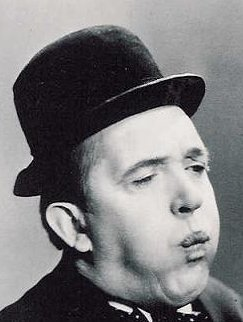
\includegraphics[width=0.7\columnwidth] {../images/SLaurel.jpg}
  \end{center}
  \caption{Que préférer ? Le gout, la couleur ou les deux ?  }
  \label{fig:gouts}
\end{figure}

Nous avons donc travaillé sur le concept de Edge Computing permettant de fournir de la puissance de calculs beaucoup plus bas dans le réseau et au plus proche des utilisateurs. L'intérêt est donc double, à la fois désengorger le réseau mais aussi diminuer la latence.
Dans ce concept notre but est d’évaluer une solution open source : OpenEdgeComputing et de la mettre en oeuvre en proposant des outils spécifiques au besoin de notre client.

Notre critère d’évaluation se pose sur les rapports d’état de l’art de notre recherche. En effet, ayant partis dans plusieurs références bibliographiques repositories de code, nous devons former notre opinion sur l’état de l’art de chaque concept étudié, ainsi que leur faisabilité en prenant compte des ressources de logiciel open source à notre disposition.

\section{Contexte technique}

Dans le cadre de ce sujet, il peut-être utile de définir ou de rappeler certaines notions indispensables à la compréhension du projet : 
\begin{itemize}
\item Cloud computing
Ici la notion principale du cloud computing qui nous intéresse est l’IAAS, traduction de “infrastructure as a service”, elle consiste 
\item Edge computing
\begin{itemize}
\item Cloudlet
\item OpenEdgeComputing
\end{itemize}
\item OpenStack
\end{itemize}

\section{Méthode} 

Notre projet s’est déroulé en 3 phases distinctes : 

\begin{itemize}
\item Recherche sur edge computing et plus spécifiquement sur le projet open source OpenEdgeComputing;
\item Mise en place du projet OpenEdgeComputing;
\item Mise en place de notre propre solution.
\end{itemize}

\subsection{Recherche sur OpenEdgeComputing}

La première partie de notre projet consistait à l’étude des différents projets EdgeComputing, et plus précisément celui de OpenEdgeComputing. Nous avons étudié l’architecture général des différents projets EdgeComputing (cf. figure représentant l’architecture).

\subsection{Mise en place de OpenEdgeComputing}

Nous avons mis en place le projet qui se base en grande partie sur le projet OpenStack qui permet de gérer un ensemble de serveur afin de constituer un cloud utilisable et manageable.
Le projet OpenEdgeComputing est en quelque sorte une surcouche d’Openstack simplifiant son utilisation avec des cloudlets en apportant quelques nouvelles fonctionnalitées : 
La synthèse de machines virtuelles (VM Synthesis)
Une gestion de la continuité de certaines machines virtuelles (VM handoff)
Cartographie des Cloudlets pour sélectionner le plus proche (Discovery)

\begin{figure}[htpb]
  \begin{center}
    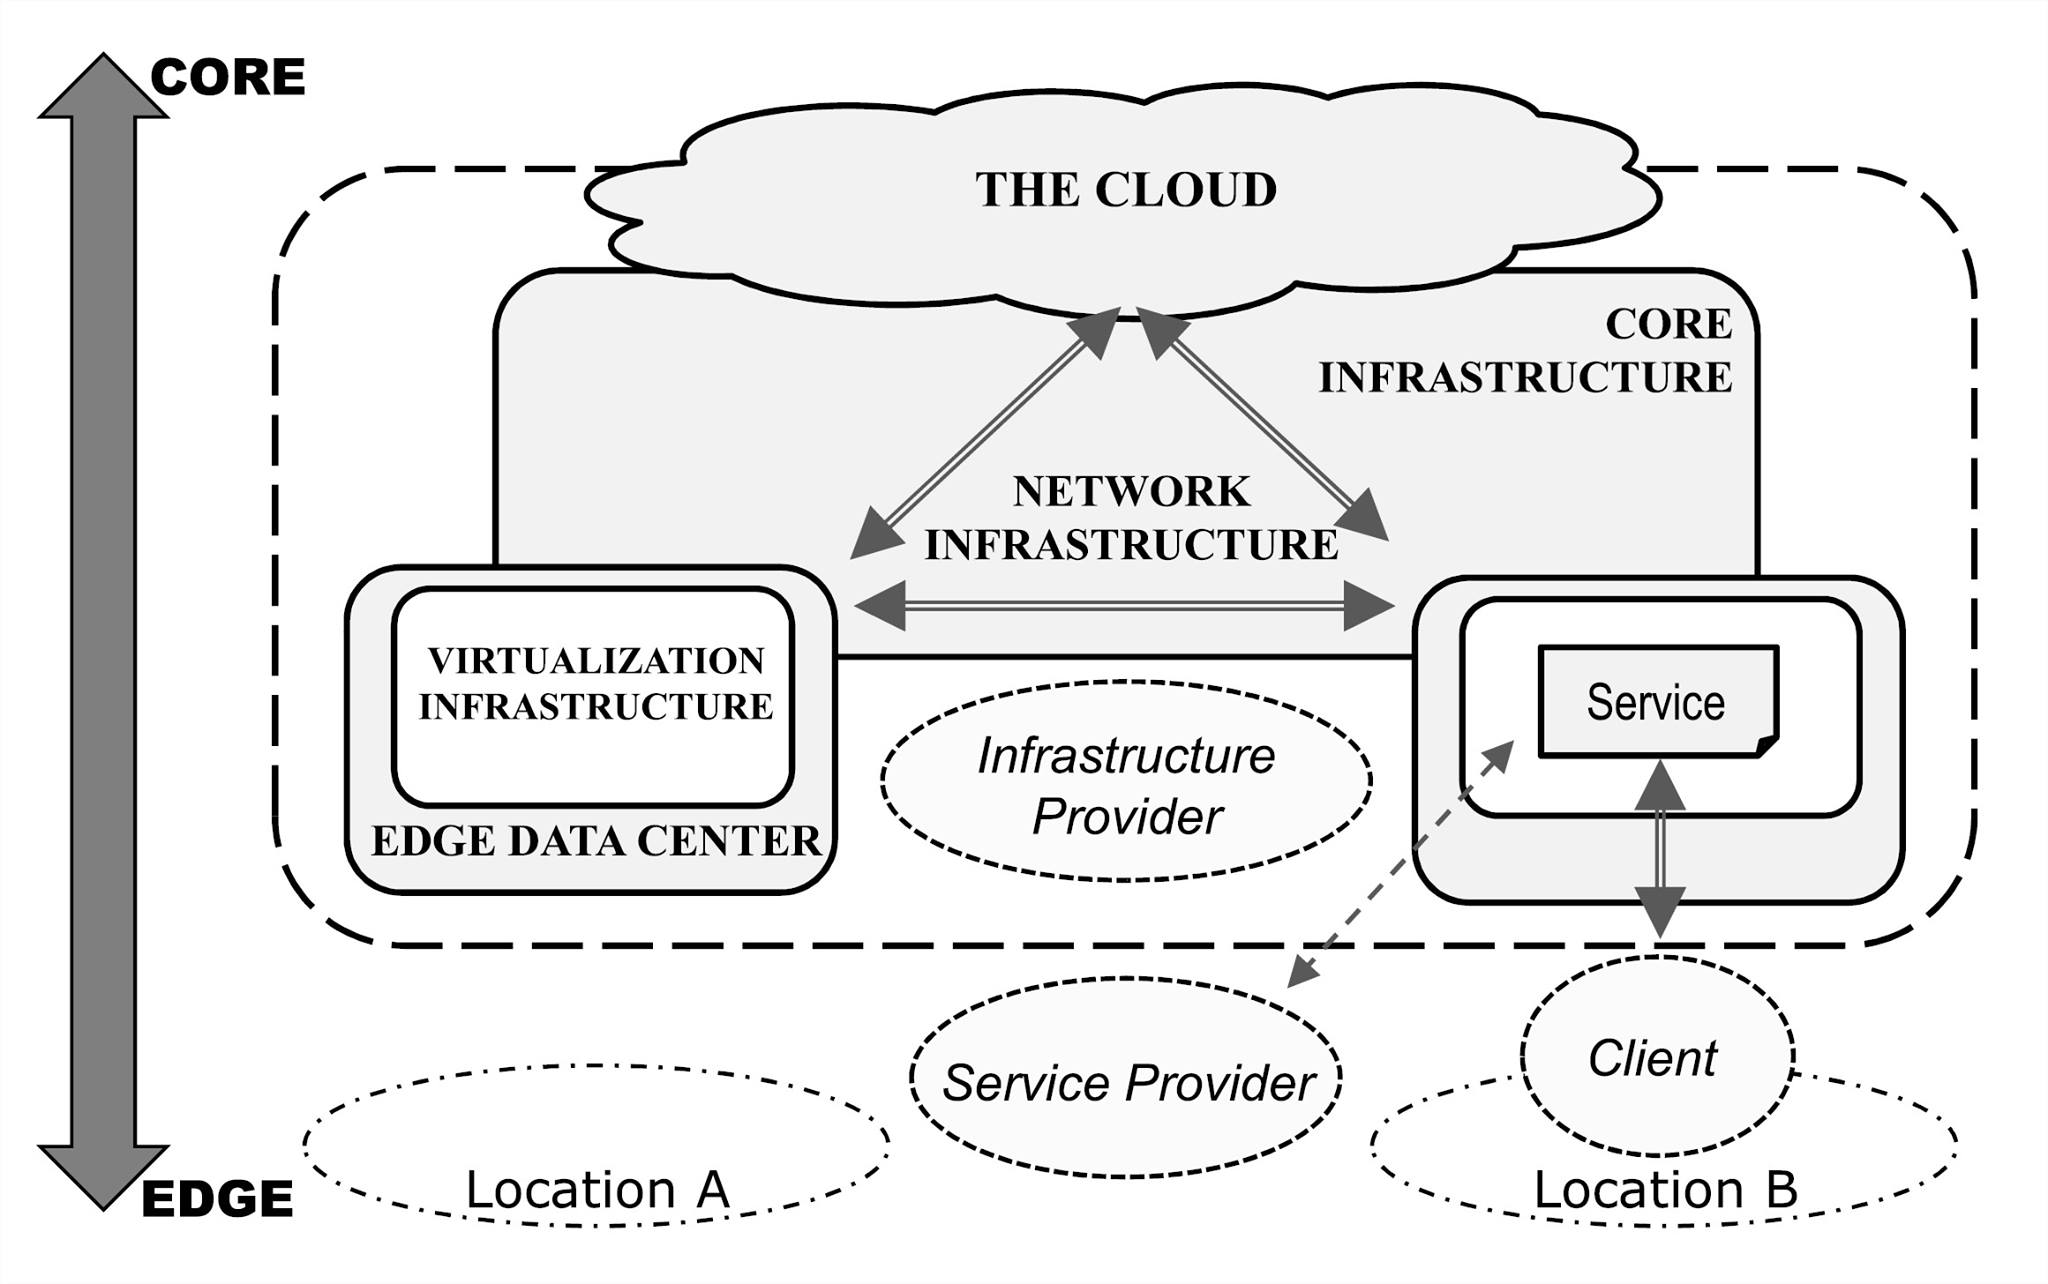
\includegraphics[width=0.8\columnwidth] {../images/open_edge.jpg}
  \end{center}
  \caption{Que préférer ? Le gout, la couleur ou les deux ?  }
  \label{fig:gouts}
\end{figure}

La première partie consiste à installer Openstack Kilo, ensuite le projet OpenEdgeComputing possède plusieurs parties qui sont liées aux différentes fonctionnalitées ajoutées. La première à installer est la synthèse de machines virtuelle, elle consiste en l’installation d’une version modifiée de qemu ainsi que d’outils permettant la gestion de la synthèse de machines virtuelles.
La deuxième partie consiste en une modification de l’interface d’openstack, qui inclut désormais la gestion des cloudlets.

\subsection{Mise en place de notre solution}

Nous avons finalement mis en place notre solution. Nous avons discuté de l’architecture général de notre application avec M. LE TOQUIN. (cf figure de notre architecture).

\begin{figure}[htpb]
  \begin{center}
    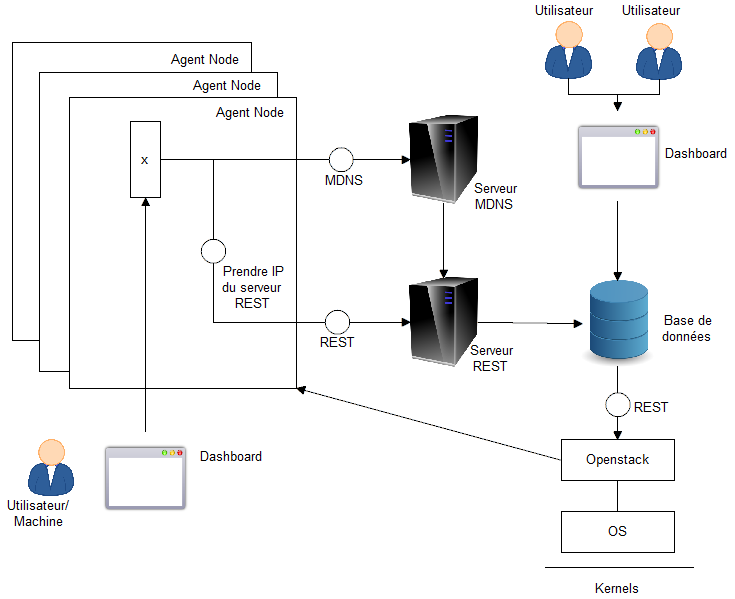
\includegraphics[width=0.7\columnwidth] {../images/schema_architecture.png}
  \end{center}
  \caption{Que préférer ? Le gout, la couleur ou les deux ?  }
  \label{fig:gouts}
\end{figure}

Nous pouvons distinguer deux parties dans cette architecture.
La partie OpenStack
La partie applicative

\subsubsection{Langage : Python}

Nous avons choisi d’utiliser le langage Python pour sa simplicité et sa mise en oeuvre rapide et efficace pour une architecture légère. Ses performances sont suffisantes pour l’application déployé.

\subsubsection{Gestion du cloud : Agent OpenStack}

L’agent OpenStack permet une connection à une infrastructure Openstack et une gestion de certains processus de virtualisation afin de pouvoir utiliser la puissance des équipements sur lesquels cet agent est installé, comme un noeud nova-compute standard. Un noeud nova-compute permet d'exécuter des machines virtuelles sur un ordinateur, sous la supervision d’OpenStack. Cet agent est basé sur docker ainsi que sur ubuntu 10.04:
Ce choix est basé sur deux choses :
\begin{itemize}
	\item Docker permet un déploiement rapide et sans dépendance logicielle autre que lui-même
	\item Ubuntu 14.04 est la version imposé par le projet OpenEdgeComputing, car celui-ci ne fonctionne que sur cette distribution linux.
\end{itemize}

Le fonctionnement de cet agent est le suivant : 
\begin{itemize}
	\item Il va dans un premier temps récupérer l’adresse ip du serveur OpenStack qui lui correspond via l’agent node.
	\item Puis il va s’y connecter pour pouvoir offrir sa puissance de calcul à l’infrastructure OpenStack.
\end{itemize}
\subsubsection{Interface utilisateur : Agent Node}

L’interface utilisateur appelé Agent Node permet à un utilisateur de notre application de pouvoir venir mettre des ressources matérielles à disposition. Pour cela une interface listant tous les objets compatibles avec le cloud et OpenStack est à sa disposition. (cf figure interface) En venant cliquer sur le bouton “NOM DU BOUTON”, l’utilisateur enregistre directement son appareil dans la base de donnée où se trouve toutes les ressources disponibles sur le cloud d’Orange. Pour cela nous avons utilisé un serveur REST ainsi qu’un serveur mDNS détaillé ci-dessous.

\subsubsection{Processus de découverte : mDNS}

Lorsqu’un utilisateur se connecte à notre interface, il doit pouvoir mettre à disposition les ressources qu’il souhaite. Pour ce faire, la première étape consiste en la découverte du serveur REST ainsi qu’en la découverte du serveur OpenStack. Le protocole mDNS-SD signifie multicast Domain Name Service - Service Discovery. Il s’agit une mécanisme de adresser les messages dans le réseau sans savoir à quel périphérique étranger qu’on communique (mDNS), ainsi que la découverte de services (Service Discovery). En prenant compte des conseils de M. Letoquin, nous avons utilisé la bibliothèque zeroconf écrite en Python. La solution zeroconf permet de découvrir de manière simple les services se situant sur le même réseau. Nous avons donc implémenté un serveur mDNS permettant de publier le service du serveur REST, transmettre les informations de ce serveur et du serveur OpenStack sur le réseau. Un simple script permet ensuite à notre Agent Node la découverte de ces serveurs et de communiquer avec.

\subsubsection{Serveur REST}

Une fois la découverte effectué, afin que l’utilisateur puisse mettre à disposition ses appareils, il doit pouvoir enregistrer son appareil dans la base de donnée regroupant toutes les ressources disponibles sur le réseau d’Orange. Pour ce faire, nous avons implémenté un serveur REST (representational state transfer). Un serveur REST permet de comprendre les requêtes envoyés par un client via un format défini au préalable et ensuite enregistré les données reçues dans une base de donnée. Nous avons utilisé le format Json, très utilisé et simple d’utilisation.  (cf. Exemple de json )

\begin{figure}[htpb]
  \begin{center}
    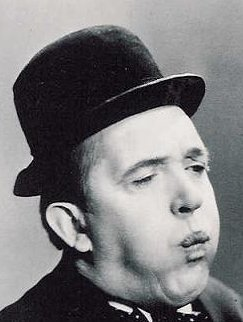
\includegraphics[width=0.7\columnwidth] {../images/SLaurel.jpg}
  \end{center}
  \caption{Exemple de JSon }
  \label{fig:gouts}
\end{figure}

\subsubsection{Affichage de la base de donnée}

Afin de pouvoir bien s’en rendre compte du bon enregistrement des appareils dans la base de donnée, nous avons créé une interface affichant la base de donnée. (cf. image dashboard)

\begin{figure}[htpb]
  \begin{center}
    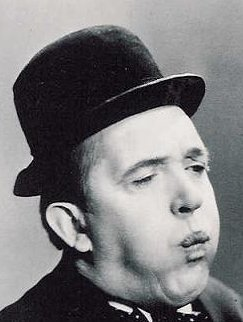
\includegraphics[width=0.7\columnwidth] {../images/SLaurel.jpg}
  \end{center}
  \caption{Représentation de notre Dashboard}
  \label{fig:gouts}
\end{figure}

\section{Résultats}

On dit un truc du genre on va diviser notre truc en 3 partie

\subsection{Recherche sur OpenEdgeComputing}

Les recherches effectués effectués sur OpenEdgeComputing n’ont pas été particulièrement convaincantes. Le projet OpenEdgeComputing est un projet universitaire assez bien documenté, cependant ce projet n’est plus maintenu depuis plus d’un an maintenant (3ans pour le code source). En plus, ce projet OpenEdgeComputing a été partiellement privatisé par les entreprises. Cela explique pourquoi nous avons une diffculté de progresser dans notre recherche. Le deuxième projet traitant de la même problématique est OpenFog cependant ce projet n’en est encore qu'à ses balbutiements, et le premier forum public de ce consortium ne se tiendra qu’en mars. 

On parle un peu de Openstack/Devstack ici ???

\subsection{Mise en place de OpenEdgeComputing}

La mise en place d’OpenEdgeComputing n’a pas été concluante en effet le manque de maintien du projet fait que de nombreux liens notamment au niveau des VMs ne sont plus disponibles. Le projet est à l’heure actuelle très difficilement exploitable et absolument pas prêt pour une quelconque mise en production.

\subsection{Mise en place de notre solution}

La solution que nous avons mise en oeuvre est concluante et fonctionne bien d’un point de vue logique à petite échelle. Il faudrait cependant déployer notre application à grande échelle afin de voir si celle-ci tient la scalabilité.

\section{Analyse}

Une importante partie de notre travail a été consacré à la découverte de Edge Computing et de l’état de l’art des existants. Cependant peu de chose ont été faites dans ce domaine et il nous a fallu repartir de 0 et implémenter notre solution. Celle-ci n’est probablement pas exploitable en l’état à grande échelle mais permet de poser les bases sur lesquelles s’appuyer pour un développement futur plus important.

\section{Discussion}

Le Edge Computing n’en est qu’à ses balbutiements, il n’y a pas encore de standard de disponible sur le marché que cela vienne d’un acteur privé ou du monde de l’open source. Cependant certains paradigmes semble revenir comme le montre l’article (scientifique traité par Merwan a retrovué et a cité). En effet, l’usage du protocole mDNS-SD est très connu dans le monde professionnel, par contre, aucun essai a été mené pour améliorer la solution cloud. Notre solution est basé sur ces paradigmes mais ne présente qu’un début de solution. Cette solution nécessite une recherche plus coûteuse en demandant d’accès à des logiciels à propriété privée.


\section{Références bibliographiques}

%\\bibliographystyle{IEEEbib} %numérique
%\bibliographystyle{utphys}
%\bibliographystyle{alpha}  %alphanumérique
%\\bibliography{bibliographie}  



\end{document}
